\section{Date: 2026-10-06}
\noindent \textbf{Series ID: PCU2212102212101122} 

\noindent This series is titled Producer Price Index by Industry: Natural Gas Distribution: Residential Natural Gas for Middle Atlantic Census Division and has a frequency of Monthly. The units are Index Jun 2012=100 and the seasonal adjustment is Not Seasonally Adjusted.The observation start date is 2012-06-01 and the observation end date is 2026-08-01.The popularity of this series is 1. \\ 

\noindent \textbf{Series ID: EFAOXFBNQ} 

\noindent This series is titled Percent of Value of Loans Made Under Participation or Syndication for All Commercial and Industry Loans, Other Risk (Acceptable), U.S. Branches and Agencies of Foreign Banks (DISCONTINUED) and has a frequency of Quarterly, 2nd Month's 1st Full Week. The units are Percent and the seasonal adjustment is Not Seasonally Adjusted.The observation start date is 2012-07-01 and the observation end date is 2017-04-01.The popularity of this series is 1. \\ 

\subsection{Raw Regression}
\noindent Regresses the two series against each other directly. A significant result here can come just as easily from both series sharing a long-run trend as from any real relationship.

\begin{center}
\begin{tabular}{lclc}
\toprule
\textbf{Dep. Variable:}                   & value\_fred\_EFAOXFBNQ & \textbf{  R-squared:         } &     0.444   \\
\textbf{Model:}                           &          OLS           & \textbf{  Adj. R-squared:    } &     0.413   \\
\textbf{Method:}                          &     Least Squares      & \textbf{  F-statistic:       } &     14.37   \\
\textbf{Date:}                            &    Tue, 06 Oct 2026    & \textbf{  Prob (F-statistic):} &  0.00134    \\
\textbf{Time:}                            &        17:29:15        & \textbf{  Log-Likelihood:    } &   -69.835   \\
\textbf{No. Observations:}                &             20         & \textbf{  AIC:               } &     143.7   \\
\textbf{Df Residuals:}                    &             18         & \textbf{  BIC:               } &     145.7   \\
\textbf{Df Model:}                        &              1         & \textbf{                     } &             \\
\textbf{Covariance Type:}                 &       nonrobust        & \textbf{                     } &             \\
\bottomrule
\end{tabular}
\begin{tabular}{lcccccc}
                                          & \textbf{coef} & \textbf{std err} & \textbf{t} & \textbf{P$> |$t$|$} & \textbf{[0.025} & \textbf{0.975]}  \\
\midrule
\textbf{const}                            &     104.3514  &       21.206     &     4.921  &         0.000        &       59.798    &      148.904     \\
\textbf{value\_fred\_PCU2212102212101122} &      -0.8266  &        0.218     &    -3.790  &         0.001        &       -1.285    &       -0.368     \\
\bottomrule
\end{tabular}
\begin{tabular}{lclc}
\textbf{Omnibus:}       &  2.921 & \textbf{  Durbin-Watson:     } &    1.600  \\
\textbf{Prob(Omnibus):} &  0.232 & \textbf{  Jarque-Bera (JB):  } &    1.265  \\
\textbf{Skew:}          &  0.146 & \textbf{  Prob(JB):          } &    0.531  \\
\textbf{Kurtosis:}      &  1.803 & \textbf{  Cond. No.          } & 1.10e+03  \\
\bottomrule
\end{tabular}
%\caption{OLS Regression Results}
\end{center}

Notes: \newline
 [1] Standard Errors assume that the covariance matrix of the errors is correctly specified. \newline
 [2] The condition number is large, 1.1e+03. This might indicate that there are \newline
 strong multicollinearity or other numerical problems.

\begin{figure}
\centering
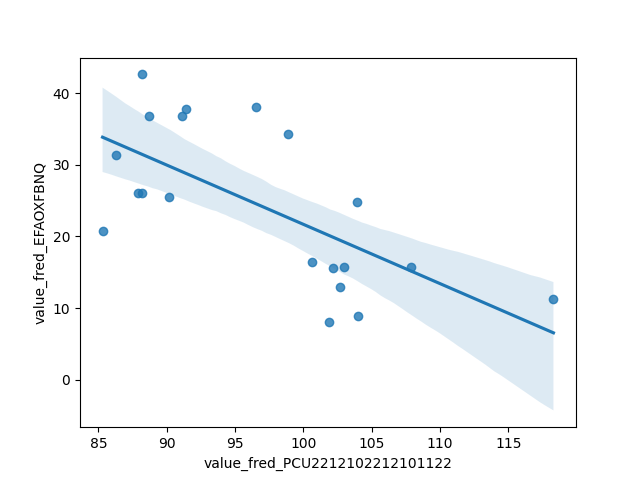
\includegraphics[scale = 0.9]{plots/plot_2026-10-06.png}
\caption{Raw Regression Plot for 2026-10-06}
\end{figure}
\newpage
\subsection{Detrended Regression}
\noindent Regresses the residuals of each series after removing its own linear time trend, so a shared trend can no longer drive the result on its own. A relationship that stays significant here is better evidence of a genuine link between the two series.

\begin{center}
\begin{tabular}{lclc}
\toprule
\textbf{Dep. Variable:}                              & value\_fred\_EFAOXFBNQ\_detrended & \textbf{  R-squared:         } &     0.019   \\
\textbf{Model:}                                      &                OLS                & \textbf{  Adj. R-squared:    } &    -0.035   \\
\textbf{Method:}                                     &           Least Squares           & \textbf{  F-statistic:       } &    0.3538   \\
\textbf{Date:}                                       &          Tue, 06 Oct 2026         & \textbf{  Prob (F-statistic):} &    0.559    \\
\textbf{Time:}                                       &              17:29:15             & \textbf{  Log-Likelihood:    } &   -69.114   \\
\textbf{No. Observations:}                           &                   20              & \textbf{  AIC:               } &     142.2   \\
\textbf{Df Residuals:}                               &                   18              & \textbf{  BIC:               } &     144.2   \\
\textbf{Df Model:}                                   &                    1              & \textbf{                     } &             \\
\textbf{Covariance Type:}                            &             nonrobust             & \textbf{                     } &             \\
\bottomrule
\end{tabular}
\begin{tabular}{lcccccc}
                                                     & \textbf{coef} & \textbf{std err} & \textbf{t} & \textbf{P$> |$t$|$} & \textbf{[0.025} & \textbf{0.975]}  \\
\midrule
\textbf{const}                                       &   -4.379e-12  &        1.807     & -2.42e-12  &         1.000        &       -3.796    &        3.796     \\
\textbf{value\_fred\_PCU2212102212101122\_detrended} &      -0.2983  &        0.502     &    -0.595  &         0.559        &       -1.352    &        0.755     \\
\bottomrule
\end{tabular}
\begin{tabular}{lclc}
\textbf{Omnibus:}       &  0.524 & \textbf{  Durbin-Watson:     } &    1.639  \\
\textbf{Prob(Omnibus):} &  0.770 & \textbf{  Jarque-Bera (JB):  } &    0.580  \\
\textbf{Skew:}          &  0.060 & \textbf{  Prob(JB):          } &    0.748  \\
\textbf{Kurtosis:}      &  2.175 & \textbf{  Cond. No.          } &     3.60  \\
\bottomrule
\end{tabular}
%\caption{OLS Regression Results}
\end{center}

Notes: \newline
 [1] Standard Errors assume that the covariance matrix of the errors is correctly specified.

\begin{figure}
\centering
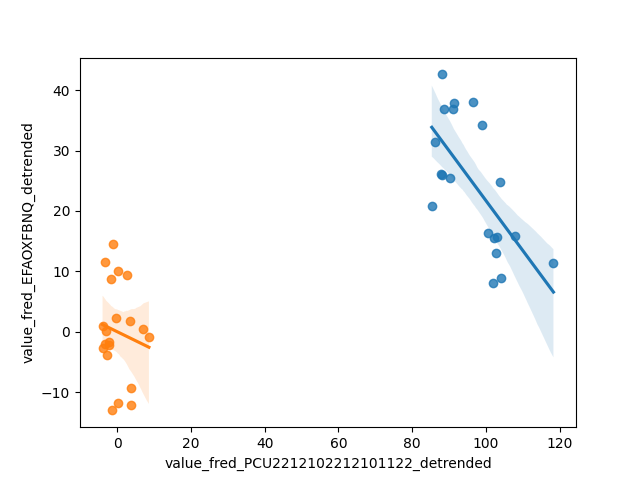
\includegraphics[scale = 0.9]{plots/plot_2026-10-06_detrended.png}
\caption{Detrended Regression Plot for 2026-10-06}
\end{figure}
\newpage
